\section{Results}
\label{sec:results}

% \begin{figure}
% 	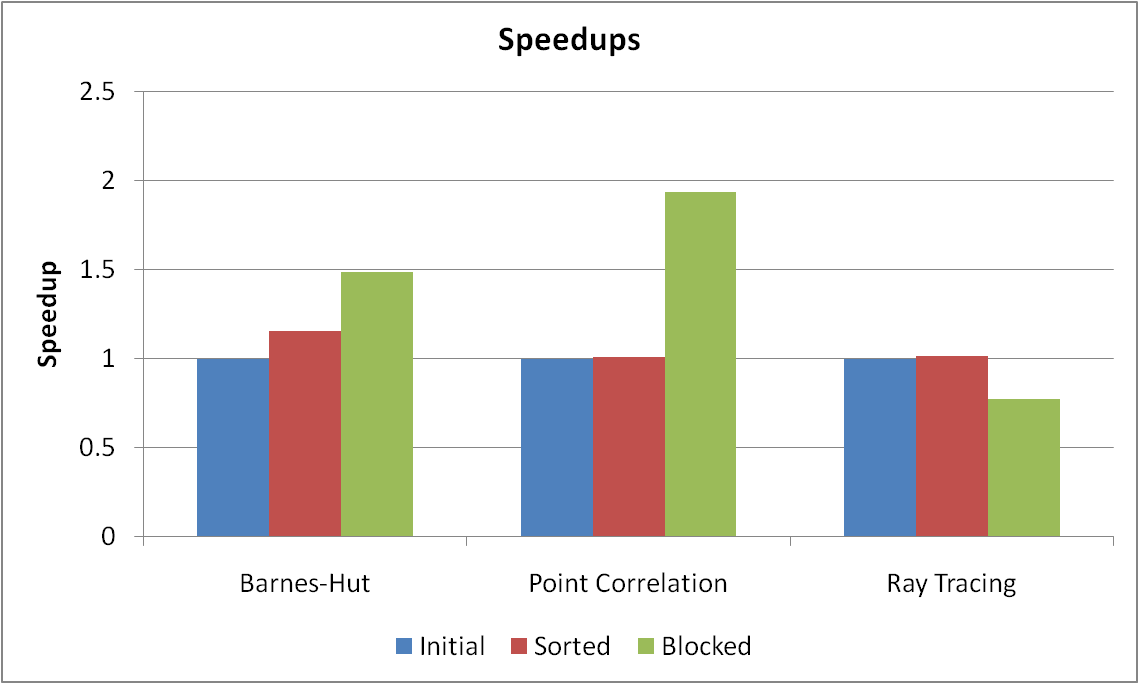
\includegraphics{speedup.png}
% 	\caption{Speedups attained using Sorting and Point Blocking for each of the three implemented examples.}
% 	\label{fig:speedups}
% \end{figure}

% BH	2.7
% PC	3.8
% RT	0.7

\Cref{fig:speedups} shows the improvements in execution time obtained with the optimizations described in this document when applied to the three implemented examples. PC got the largest speedup of 3.79 from using Sorting and Point Blocking, followed by BH with a speedup of 2.7, while the ray tracer did not achieve better execution times. To notice that the PC algorithm did not benefit at all from using only Sorting. This can be easily explained by the input generator, which was copied from the BH original implementation in Galois, and may not be suitable for the PC problem. The lack of speedup in the RT example can be easily explained by the increased complexity behind managing the blocks.

% BH
%	L1	62%
%	L2	8%
%	L3	4%

% PC
%	L1	68%
%	L2	2%
%	L3	3%

% RT
%	L1	82%
%	L2	54%
%	L3	63%

% \begin{figure}
% 	\includegraphics{misses-l1.png}
% 	\includegraphics{misses-l2.png}
% 	\includegraphics{misses-l3.png}
% 	\caption{Cache misses occurred with the base version and using the two optimizations for each of the described examples.}
% 	\label{fig:misses}
% \end{figure}

Despite the RT not achieving a better execution time, \cref{fig:misses} shows that it benefited from the described optimizations. The reported speedups can also be justified by a significant decrease in cache misses in every level due to the increase of locality. The \crefname{fig:misses} shows decreases of over 90\% of cache misses in PC and BH, for both L3 and L2. As for L1, BH and PC decreased cache misses in 38\%and 32\%, respectively. The RT algorithm showed improvements of 28\%, 46\% and 37\% for L1, L2 and L3 respectively.